\section{Results}
\label{sec:results}

\para{Main outcome.} Iterative rejection does not improve detector evasion over one-shot rewriting in this run. Across all detector-source pairs, mean paired differences are positive (iterative minus one-shot), so iterative outputs are more AI-like on average.

\begin{table*}[t]
\centering
\resizebox{\textwidth}{!}{%
\begin{tabular}{@{}llcccc@{}}
\toprule
\textbf{Source} & \textbf{Condition} & \textbf{Word detector} $\downarrow$ & \textbf{Stylometric detector} $\downarrow$ & \textbf{Mean words} & \textbf{Mean TTR} \\
\midrule
Fresh & Baseline & 0.6288 & 0.5902 & 163.7 & 0.6244 \\
Fresh & \oneshot & \textbf{0.5835} & \textbf{0.5296} & 147.3 & \textbf{0.6864} \\
Fresh & \iterative (final) & 0.5883 & 0.5644 & 146.9 & 0.6608 \\
Fresh & Human reference & 0.5613 & 0.4234 & 69.0 & 0.7946 \\
\midrule
External & Original external & \textbf{0.4926} & \textbf{0.3930} & 527.3 & 0.5049 \\
External & \oneshot & 0.5363 & 0.4425 & 184.2 & \textbf{0.6783} \\
External & \iterative (final) & 0.5389 & 0.5085 & 187.2 & 0.6707 \\
\bottomrule
\end{tabular}%
}
\caption{Condition-level summary from 30 paired items (15 fresh, 15 external). Lower detector probability indicates more detector evasion. Best values within each source block for detector scores are in \textbf{bold}.}
\label{tab:condition_summary}
\end{table*}

\begin{table*}[t]
\centering
\resizebox{\textwidth}{!}{%
\begin{tabular}{@{}llcccccc@{}}
\toprule
\textbf{Detector} & \textbf{Source} & \textbf{Mean diff} & \textbf{$p$ (t)} & \textbf{$p$ (FDR)} & \textbf{Cohen's $d$} & \textbf{95\% CI} & \textbf{Direction} \\
\midrule
\worddet & Fresh & +0.0048 & 0.7009 & 0.8645 & +0.101 & [-0.0181, 0.0281] & Worse \\
\worddet & External & +0.0025 & 0.8645 & 0.8645 & +0.045 & [-0.0241, 0.0307] & Worse \\
\styledet & Fresh & +0.0348 & 0.0414 & 0.0828 & +0.580 & [0.0063, 0.0645] & Worse \\
\styledet & External & +0.0660 & 0.0110 & \textbf{0.0440} & +0.756 & [0.0241, 0.1088] & Worse \\
\bottomrule
\end{tabular}%
}
\caption{Paired tests for \iterative final versus \oneshot (difference = iterative $-$ one-shot). Positive differences indicate that iterative rejection is more AI-like and therefore worse for evasion.}
\label{tab:paired_tests}
\end{table*}

\begin{table*}[t]
\centering
\resizebox{\textwidth}{!}{%
\begin{tabular}{@{}llcccc@{}}
\toprule
\textbf{Metric} & \textbf{Detector} & \textbf{Fresh baseline} & \textbf{Fresh one-shot} & \textbf{Fresh iterative} & \textbf{External one-shot / iterative} \\
\midrule
Pass rate @ 0.5 $\uparrow$ & \worddet & 0.067 & 0.333 & 0.333 & 0.333 / 0.333 \\
Pass rate @ 0.5 $\uparrow$ & \styledet & 0.333 & \textbf{0.467} & 0.333 & \textbf{0.600} / 0.467 \\
AUC vs human $\uparrow$ & \worddet & 0.627 & \textbf{0.520} & 0.560 & -- \\
AUC vs human $\uparrow$ & \styledet & 0.711 & \textbf{0.662} & 0.698 & -- \\
\bottomrule
\end{tabular}%
}
\caption{Decision-level effects. For pass rate, higher means more texts are classified as non-AI at threshold 0.5. For AUC versus human references, lower values indicate weaker separation; one-shot has lower AUC than iterative for both detectors.}
\label{tab:pass_auc}
\end{table*}


\begin{figure*}[t]
    \centering
    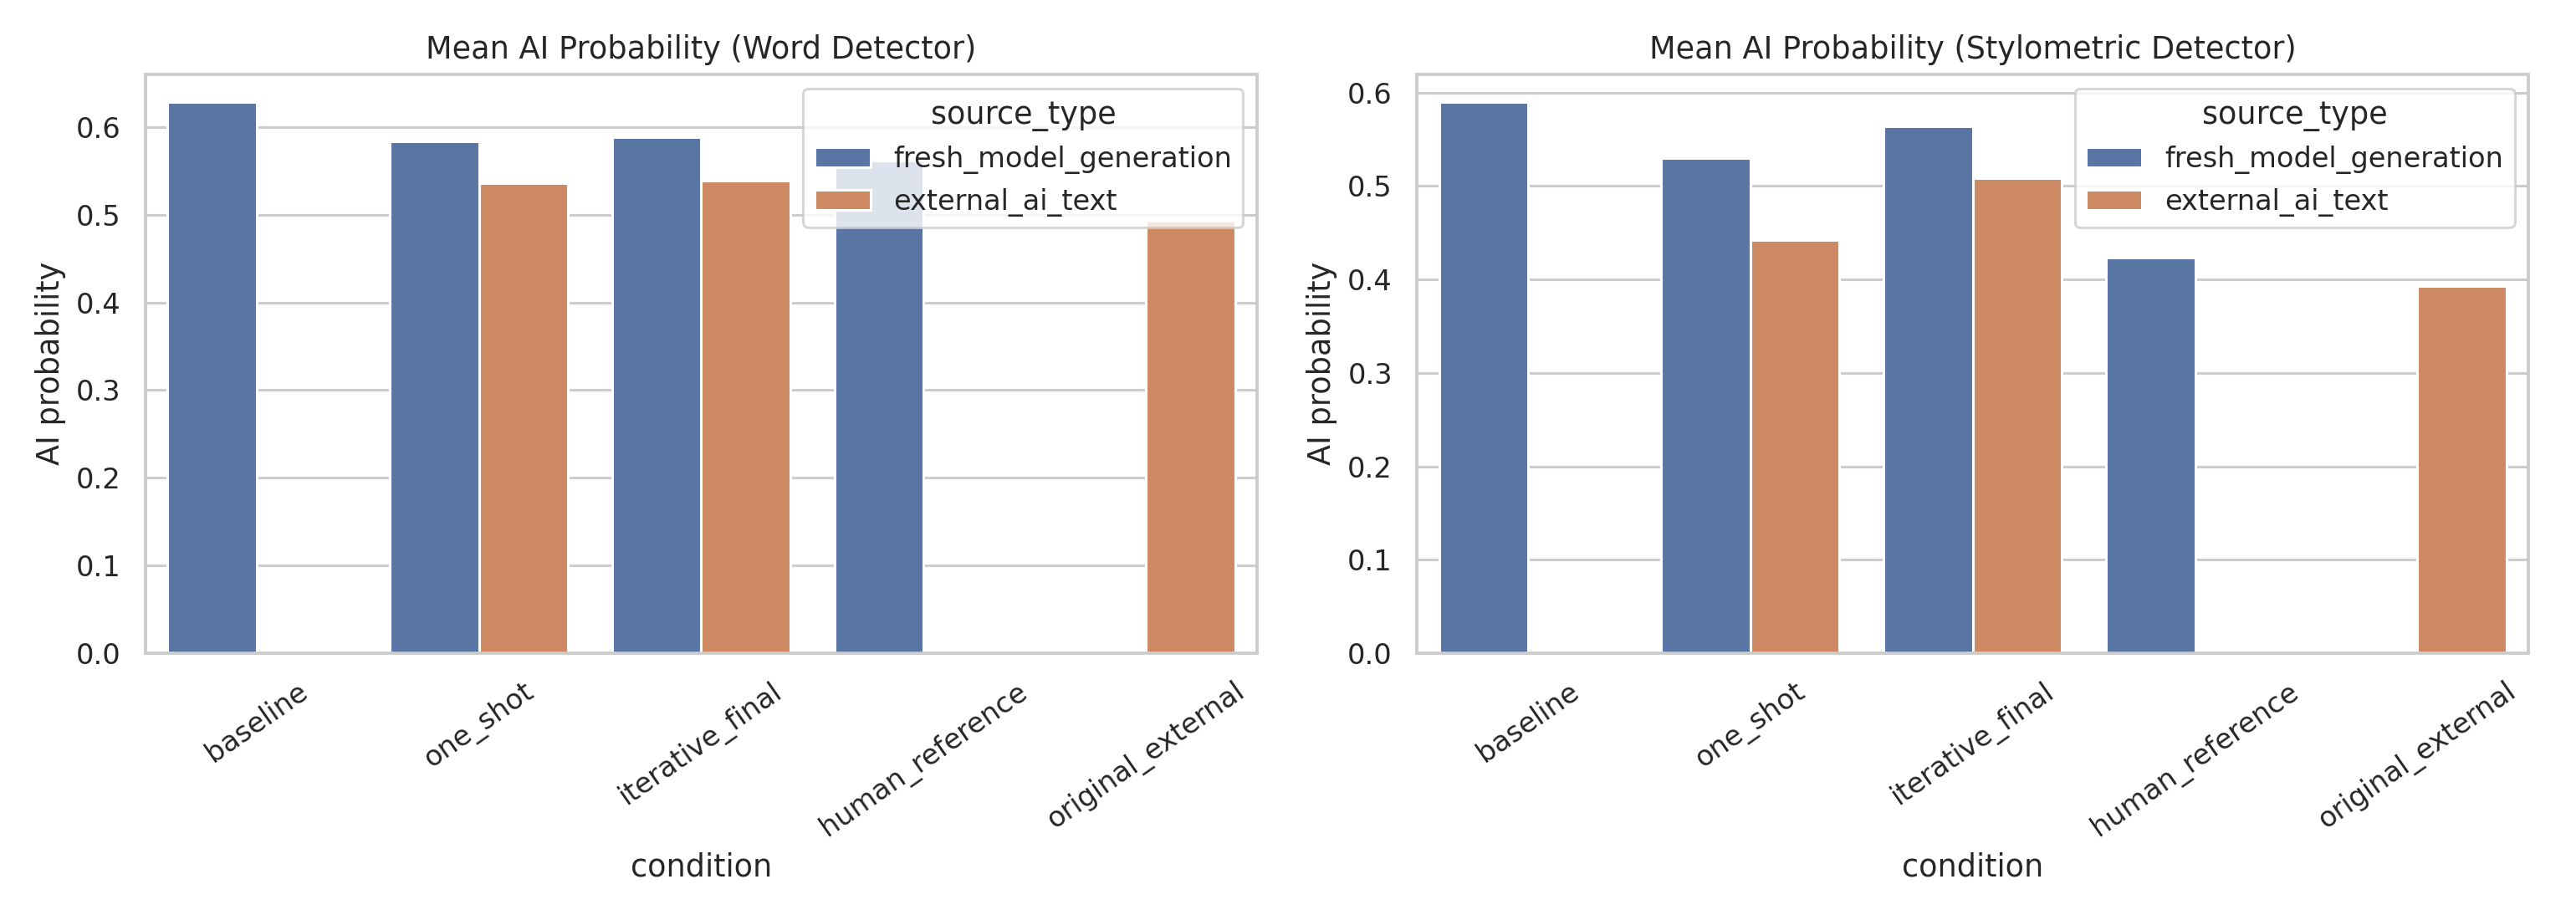
\includegraphics[width=0.95\linewidth]{figures/condition_comparison.png}
    \caption{Condition-level detector probabilities across source settings and detectors. Lower values indicate more effective evasion. \oneshot is lower than \iterative in all detector-source pairs.}
    \label{fig:condition_comparison}
\end{figure*}

\begin{figure*}[t]
    \centering
    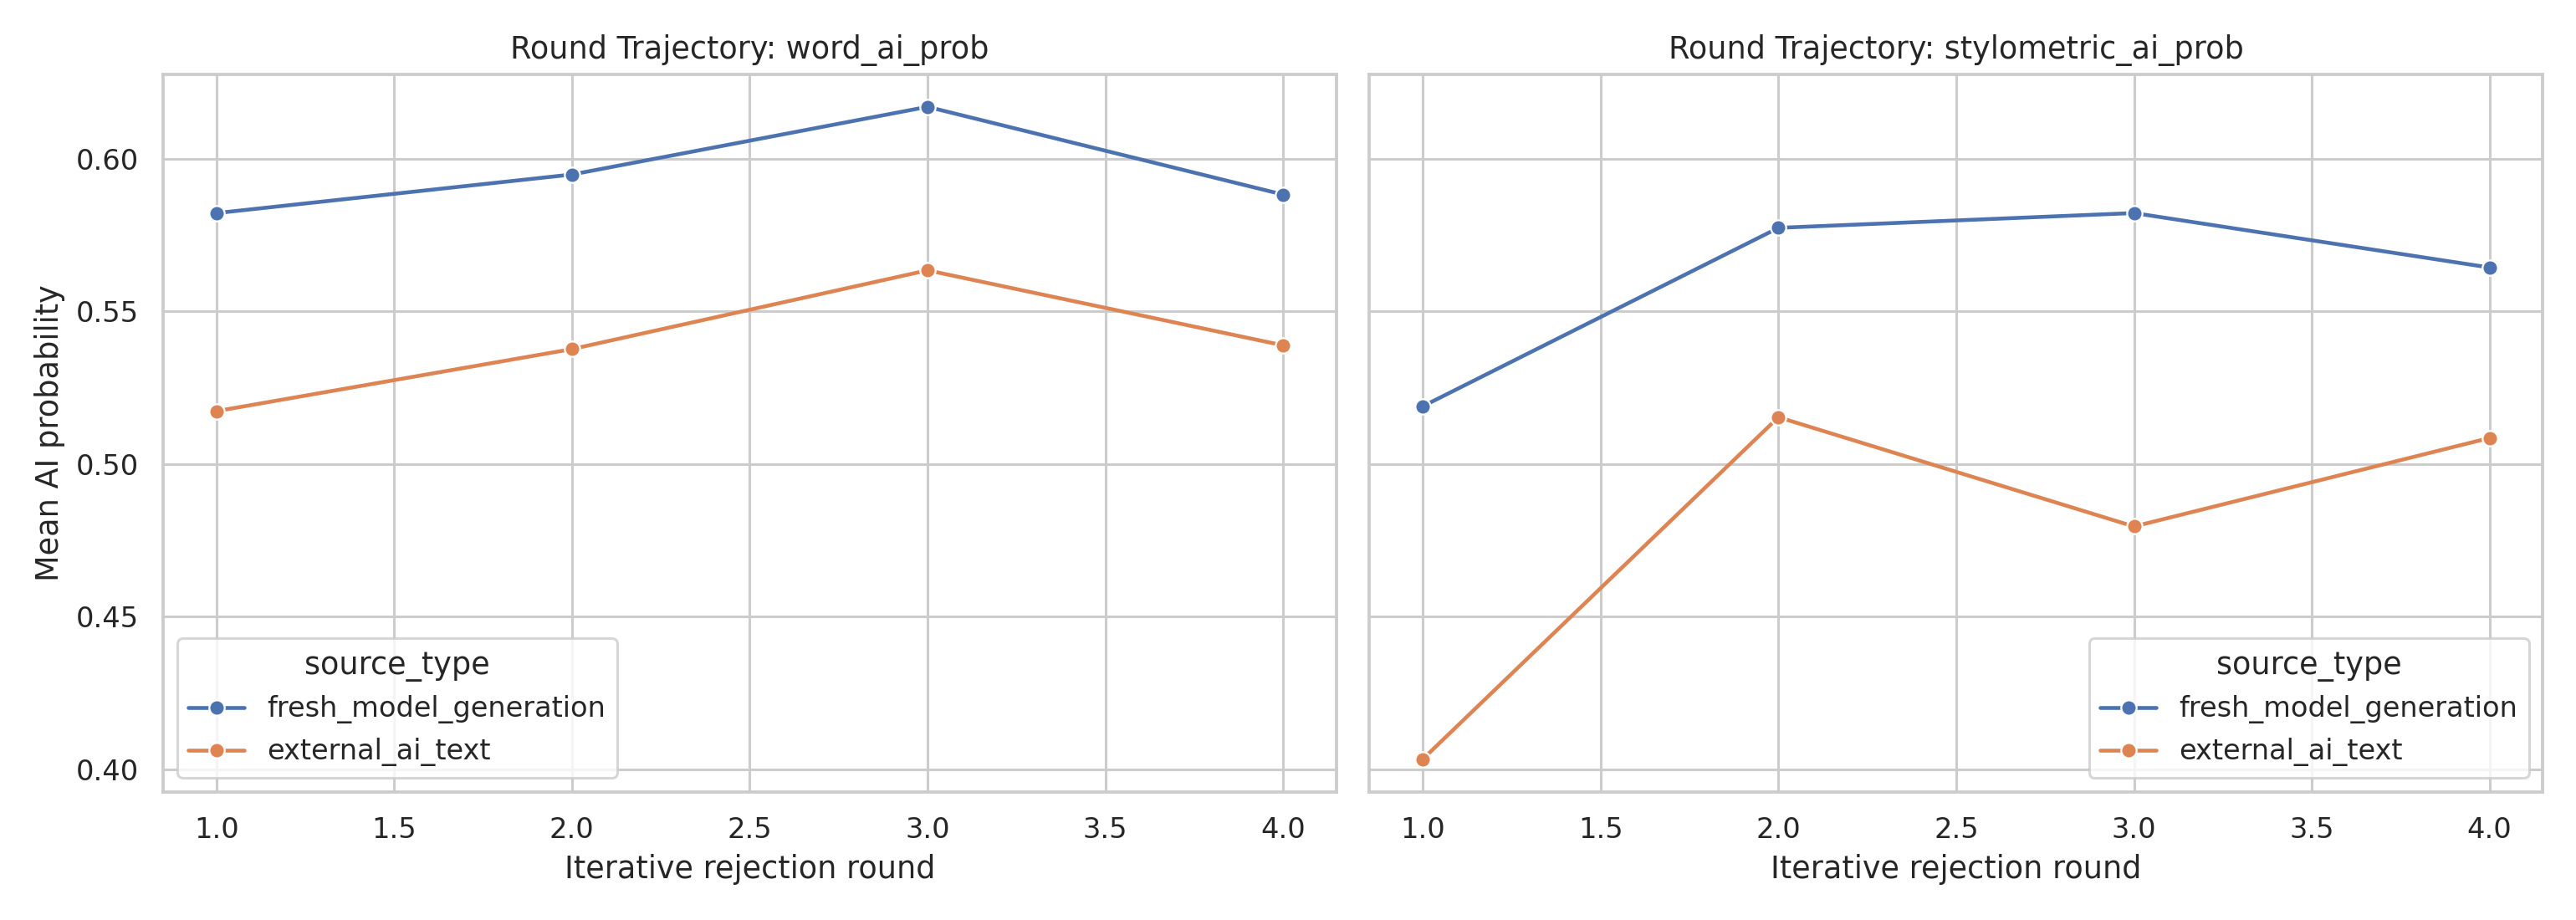
\includegraphics[width=0.95\linewidth]{figures/iterative_trajectory.png}
    \caption{Round-by-round trajectory under iterative rejection. Curves are non-monotonic and do not converge to lower final AI probability than \oneshot.}
    \label{fig:trajectory}
\end{figure*}

\begin{figure*}[t]
    \centering
    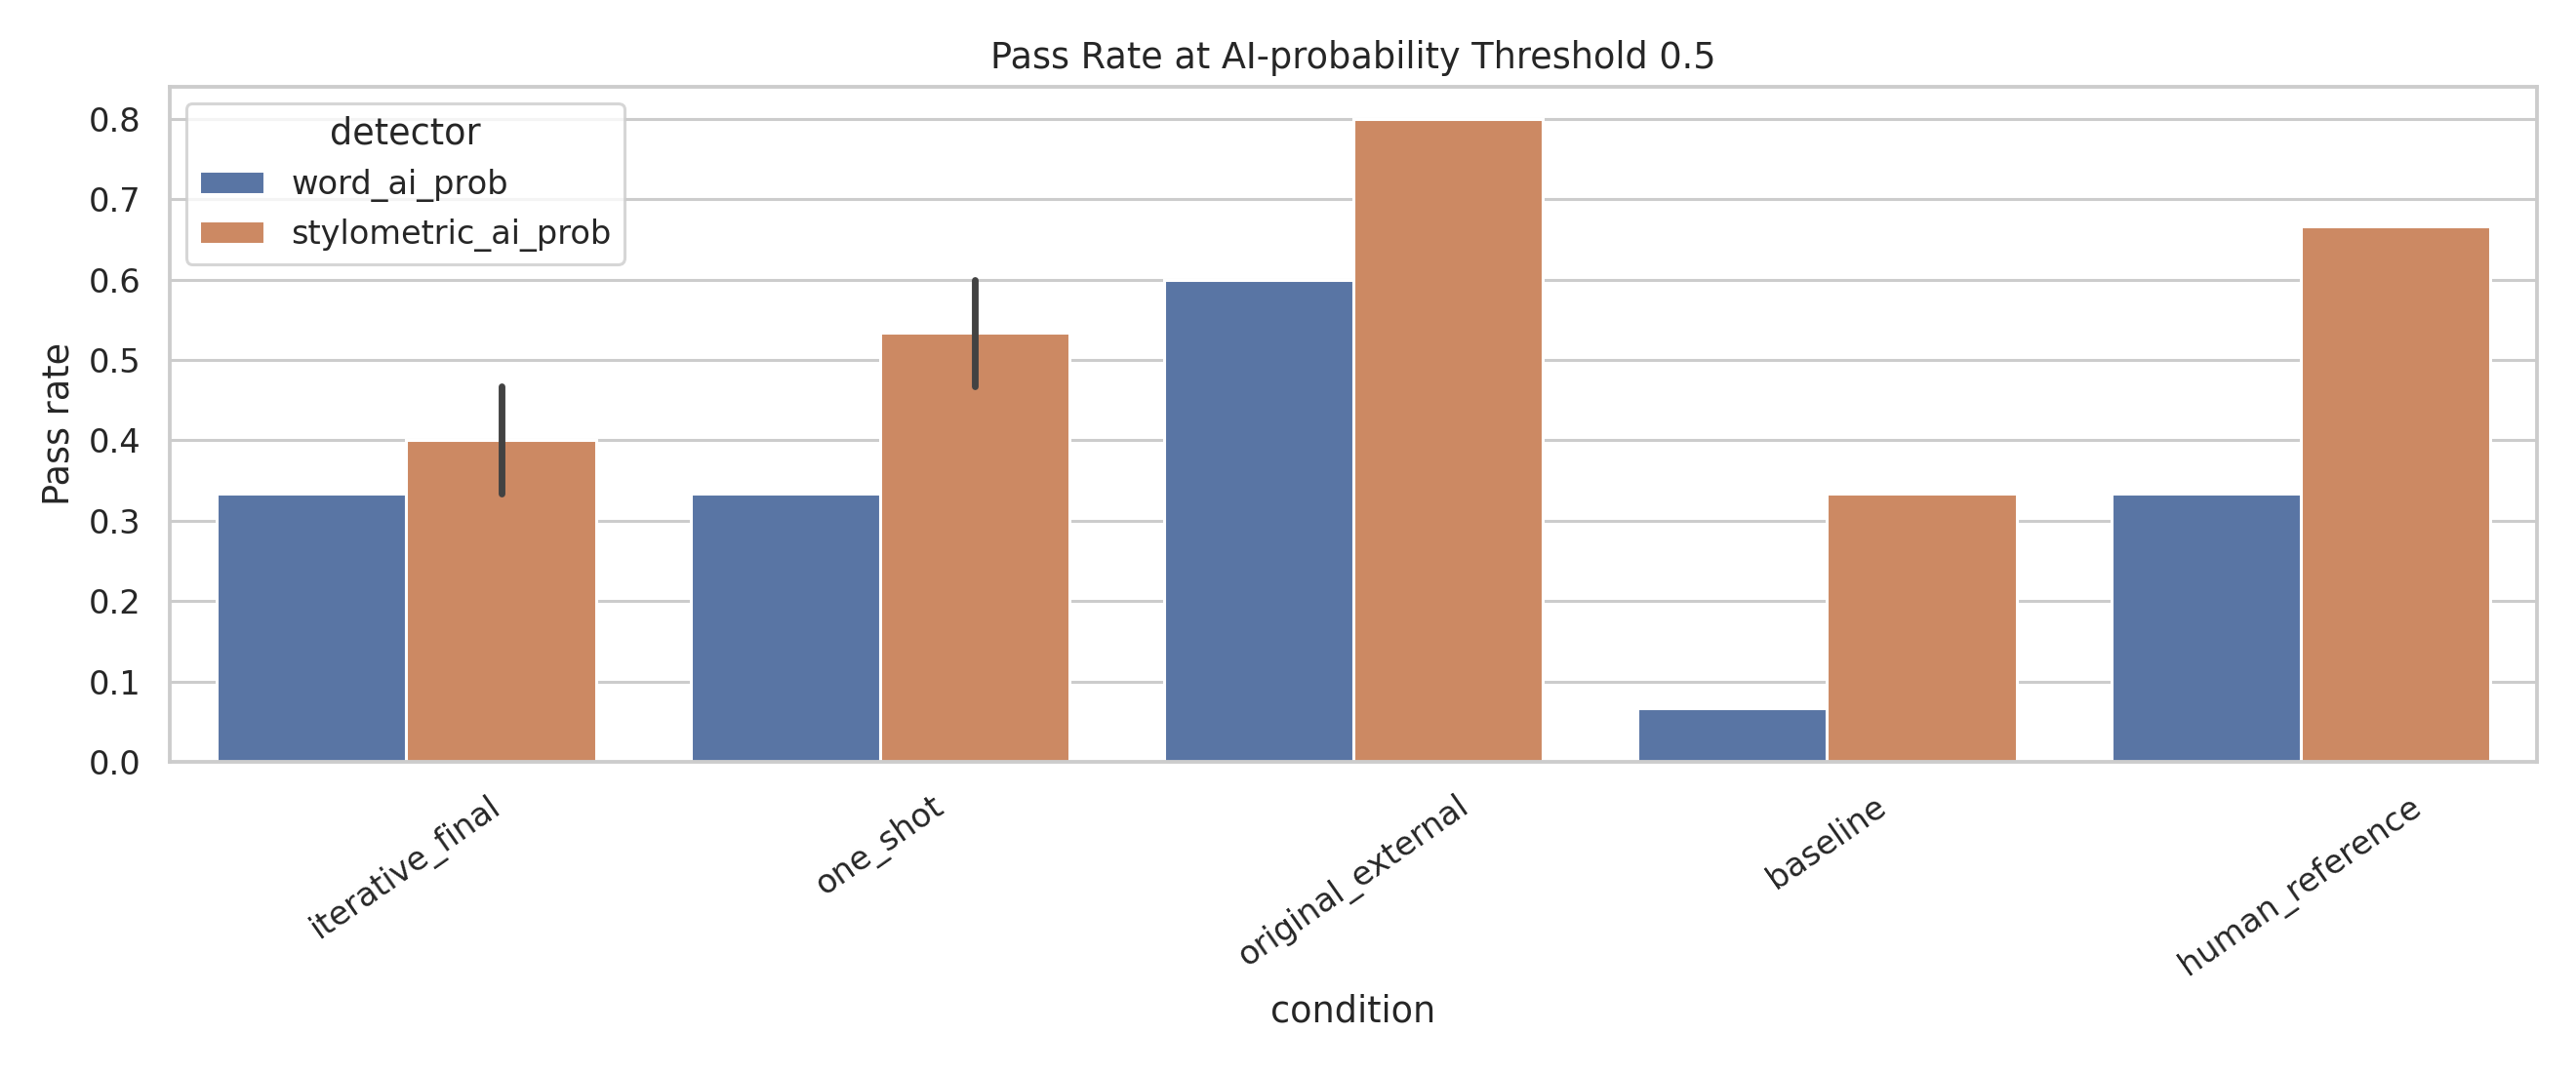
\includegraphics[width=0.95\linewidth]{figures/pass_rates.png}
    \caption{Pass rates at threshold 0.5. On the stylometric detector, iterative rejection lowers pass rate by 13.3 points relative to one-shot in both source settings.}
    \label{fig:pass_rates}
\end{figure*}

\begin{figure*}[t]
    \centering
    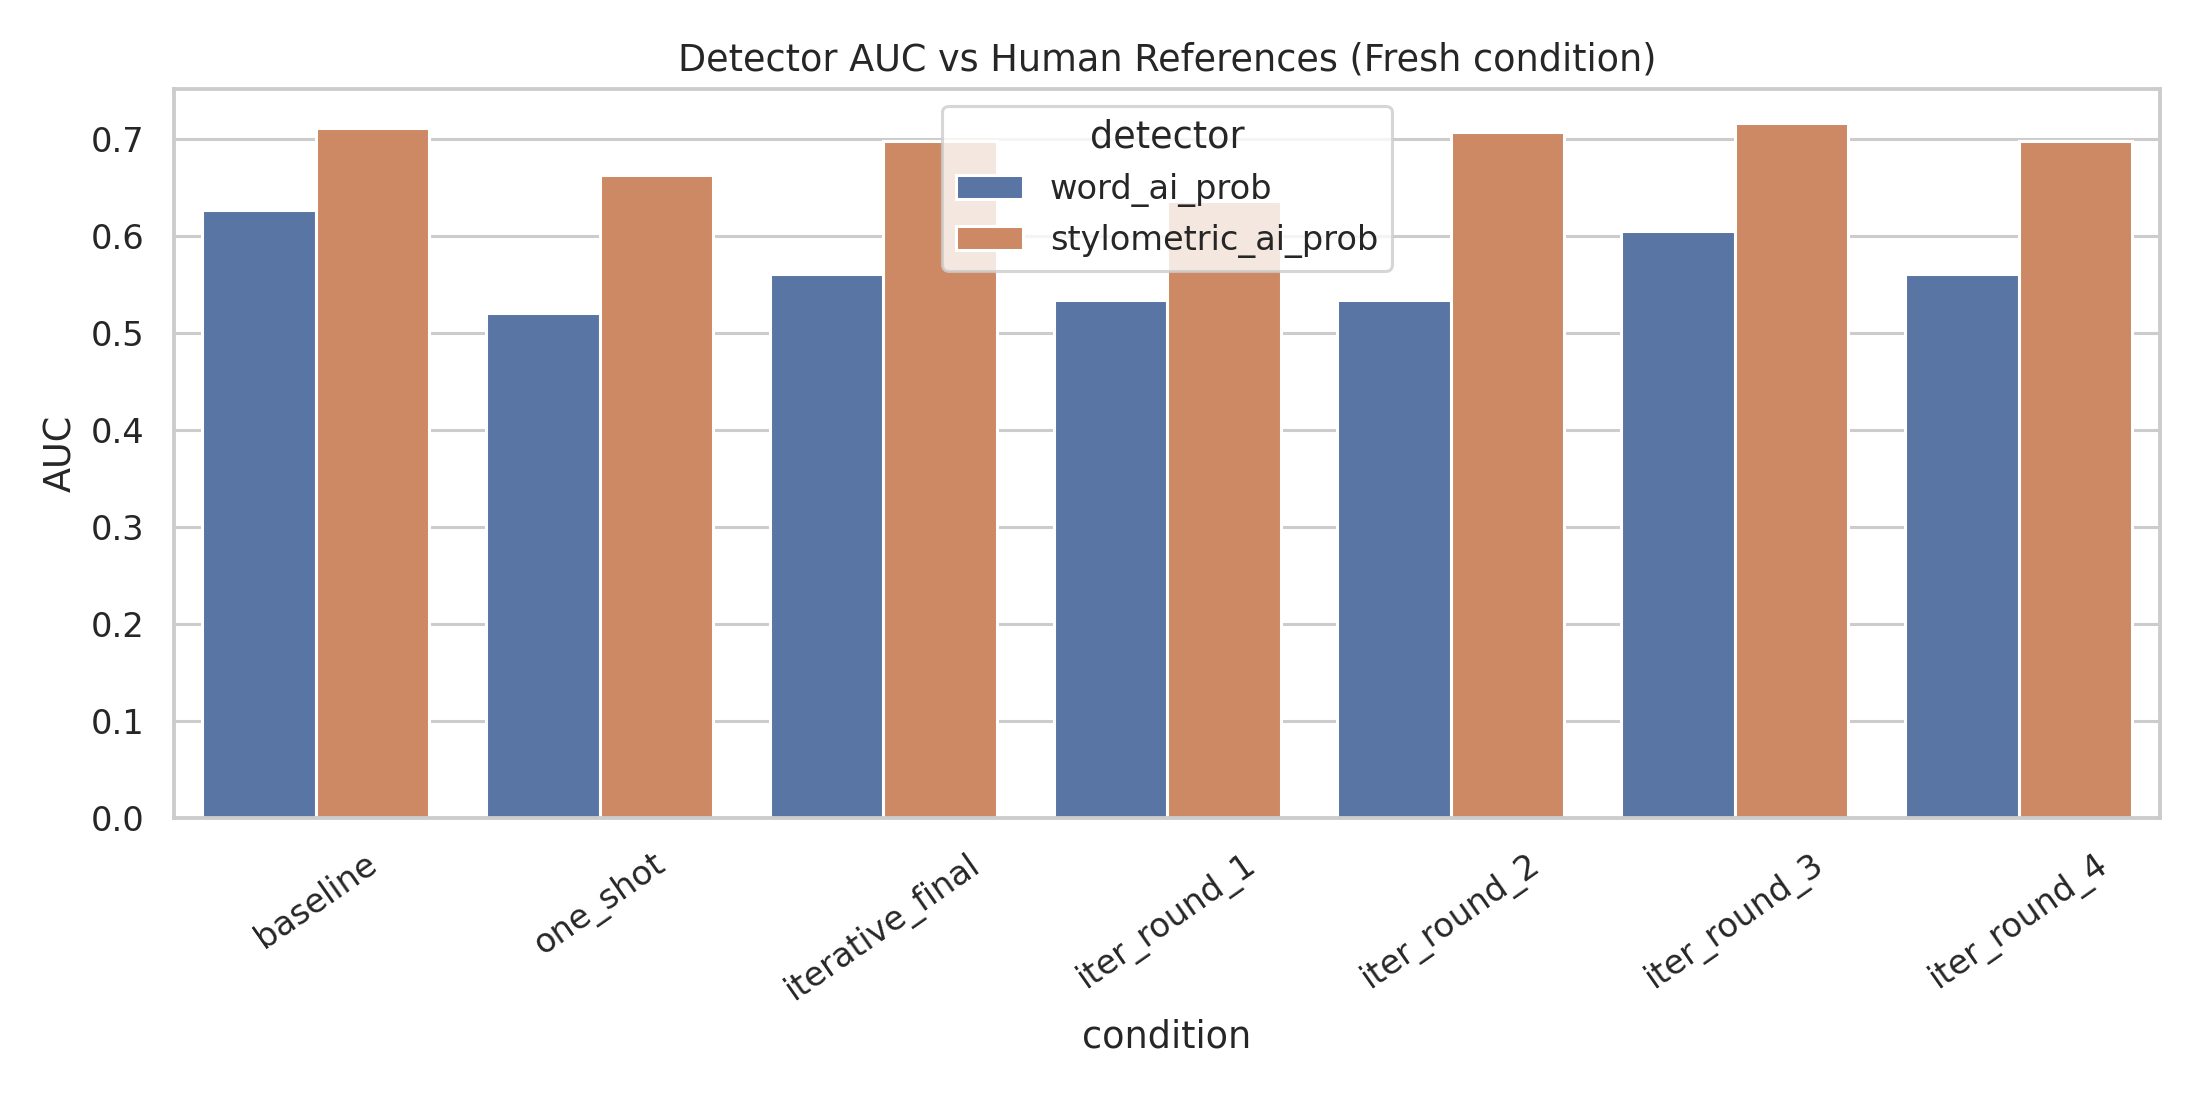
\includegraphics[width=0.95\linewidth]{figures/auc_vs_human.png}
    \caption{AUC versus human references in the fresh setting. One-shot has lower AUC than iterative for both detectors, indicating weaker detector separation under one-shot rewriting.}
    \label{fig:auc_human}
\end{figure*}

\subsection{Statistical Tests}
\tabref{tab:paired_tests} shows that the strongest effect is stylometric detection on external text: mean difference +0.0660, 95\% CI [0.0241, 0.1088], Cohen's $d=0.756$, FDR-adjusted $p=0.0440$. The fresh stylometric comparison is nominally significant before correction ($p=0.0414$) but not after FDR adjustment ($p=0.0828$). Both word-detector comparisons are small and non-significant.

\subsection{Baseline Comparisons and Trajectory}
For fresh generations, \oneshot improves over baseline on both detectors (word: 0.6288 $\rightarrow$ 0.5835; stylometric: 0.5902 $\rightarrow$ 0.5296). Iterative rewrites partially reverse that gain. For external texts, both rewrite protocols increase AI probability relative to original external text, with larger degradation for \iterative on the stylometric detector (0.5085 versus 0.4425).

Trajectory analysis shows non-monotonic behavior: some early rounds briefly reduce score, but later rounds often drift upward. This pattern suggests that repeated rejection can push style toward regularized prose features captured by stylometric detection.
